\section{Measurement instruments}
\subsection{Keithley 617 electrometer}
An electrometer is a highly sensitive instrument for electrical measurements.
When measuring voltage, it is characterized by:
\begin{itemize}
    \item High input impedance:
\SI{200}{\tera\ohm} in parallel with $<$\SI{2}{\pico\farad}
\item High precision: $\pm0.05\%$
\item High resolution: under \SI{10}{\micro\volt}
\end{itemize}
\begin{figure}[p]
    \begin{subfigure}[b]{\textwidth}
    \centering
        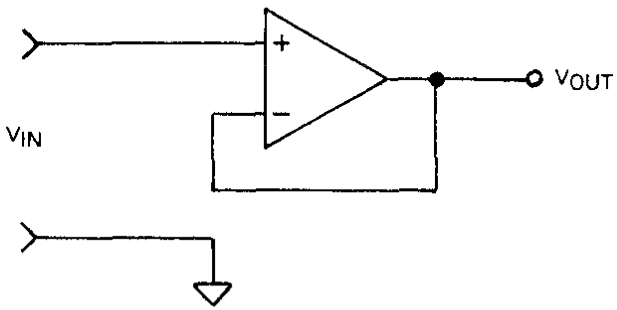
\includegraphics{figuras/instrumental/617volts.png}
        \caption{Voltage}
        %\label{fig:posicionno}
    \end{subfigure}
    \begin{subfigure}[b]{\textwidth}
    \centering
        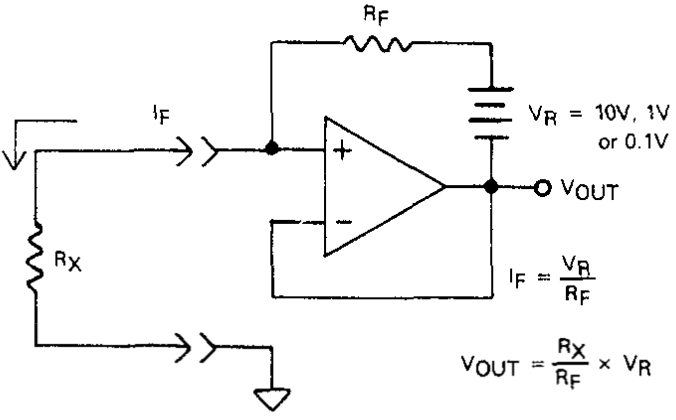
\includegraphics{figuras/instrumental/617ohms.png}
        \caption{Resistance}
        %\label{fig:posicionno}
    \end{subfigure}
    \begin{subfigure}[b]{\textwidth}
    \centering
        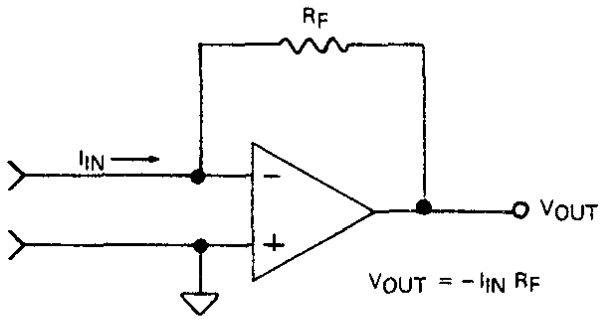
\includegraphics{figuras/instrumental/617amps.png}
        \caption{Current}
        %\label{fig:posicionno}
    \end{subfigure}
    \begin{subfigure}[b]{\textwidth}
    \centering
        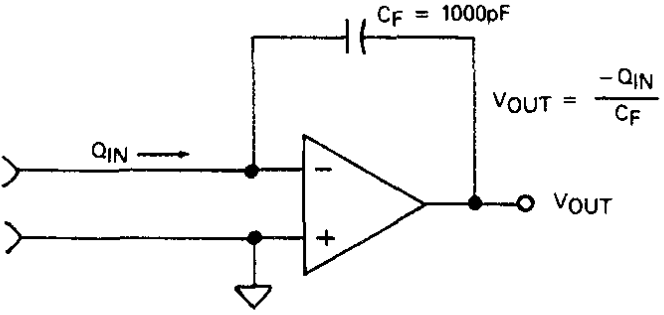
\includegraphics{figuras/instrumental/617coulombs.png}
        \caption{Charge}
        %\label{fig:posicionno}
    \end{subfigure}
    \caption{Electrometer measurement configurations.
    Reprinted from~\cite{keithley_instruments_inc._keithley_1984}.}
    \label{fig:keithley617}
\end{figure}
By adding feedback components to the input circuit,
electrometers can measure voltage, current, resistance and charge.
(\figref{fig:keithley617}).
The amplifier's high gain keeps the input terminal at 
\SI{0}{\volt}, 
which minimizes the measurement's impact on the circuit under test.
The very high input impedance,
which minimizes current drawn from the circuit under test,
is achieved partly by careful isolation of the input terminal.
For example, parts of the input circuit 
are held above the printed circuit board with teflon standoffs,
for better isolation.
\subsubsection{Guarded measurements}
When measuring voltage at high impedance nodes,
any current drawn by the measurement instrument causes a large voltage drop.
Due to the electrometer's high input impedance,
very little current is drawn through its terminals .
However, there is an additional current flow through the cables
due to the finite resistance of their insulation
(\figref{fig:unguarded}).
\fig{unguarded}{figuras/instrumental/unguarded.png}
{Effect of cable leakage on voltage measurements.
    Reprinted from~\cite{keithley_instruments_inc._keithley_1984}.}

To eliminate this leakage path,
one can use cables which surround the signal conductor with a guard (\figref{fig:guarded})
The electrometer drives the guard at the same voltage as the signal conductor.
This nulls the voltage drop across the cable insulation,
getting rid of the leakage current.
Furthermore, the effective capacitance of the cable is reduced,
as the voltage across its terminals is minimized.
\cite{rich_shielding_1983}.
\fig{guarded}{figuras/instrumental/guarded.png}
{Guarded measurement to reduce cable leakage currents.
    Reprinted from~\cite{keithley_instruments_inc._keithley_1984}.}
\subsection{Keithley 220 current source}
A current source is an instrument typically used to force current through large impedances,
like that of a MOS gate oxide.
This requires a high output impedance,
to ensure the current is flowing through the external device
and not within the instrument.
Like the electrometer,
it can be used with a guard
in order to reduce leakage currents
due to cabling or other leakage paths.
(\figref{fig:220guard}).
\begin{figure}[H]
    \begin{subfigure}[b]{\textwidth}
    \centering
        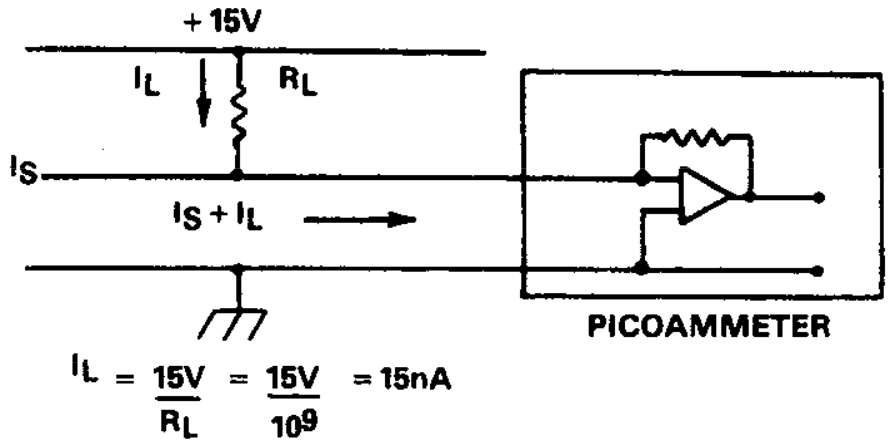
\includegraphics{figuras/instrumental/220unguarded.png}
        \caption{Unguarded.}
        %\label{fig:posicionno}
    \end{subfigure}
    \begin{subfigure}[b]{\textwidth}
    \centering
        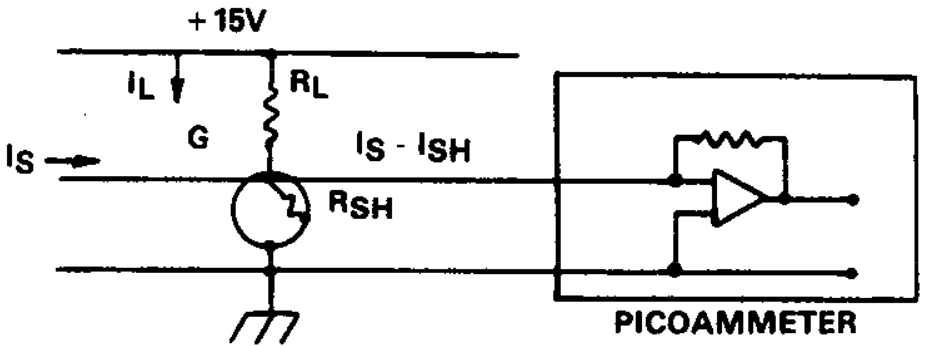
\includegraphics{figuras/instrumental/220guarded.png}
        \caption{Guarded.}
        %\label{fig:posicionno}
    \end{subfigure}
        \caption{Effect of current leakage when using a current source.
        By surrounding the signal conductor with a guard,
        leakage currents flow through the guard and do not impact the measurement.
    Reprinted from~\cite{keithley_instruments_inc._keithley_1984}.}
    \label{fig:220guard}
\end{figure}
\subsection{Keithley KUSB-3108 data acquisition module}
The Keithley KUSB-3108 data acquisition module
has multiple analog and digital inputs/outputs controlled by a PC.
With the help of external circuitry,
it can be used to carry out field measurements
where the previous instruments would not be practical
(for example, in irradiation centers far from the lab).

The Floating Gate measurement setup uses a KUSB analog input
connected to the output of a transimpedance amplifier.
The voltage at that input is proportional to the drain current
of the read transistor.

The APS measurement setup uses an analog output to control a current source driving a LED.
An analog output controls the APS Reset input,
and two analog inputs measure the APS output voltage.
